\documentclass[%
bachelor,    % тип документа
%natbib,      % использовать пакет natbib для "сжатия" цитирований
subf,        % использовать пакет subcaption для вложенной нумерации рисунков
href,        % использовать пакет hyperref для создания гиперссылок
colorlinks,  % цветные гиперссылки
%fixint,     % включить прямые знаки интегралов
]{disser}

\usepackage[
  a4paper,
  mag=1000,
  left=30mm, right=15mm, top=20mm, bottom=20mm,
  headsep=1.25cm,
  footskip=1cm
]{geometry}

\usepackage[intlimits]{amsmath}
\usepackage{amssymb,amsfonts}
\usepackage{icomma}
% Подпись под картинками
\renewcommand\thesubfigure{\asbuk{subfigure}}


\usepackage[toc]{glossaries}
\makeglossaries
%!TEX root = thesis.tex"`

\newacronym{ifg}{ИФГ}{Идеальный Ферми-газ}
\newacronym{okp}{ОКП}{Однокомпонентная плазма}
\newacronym{bpf}{БПФ}{Быстрое преобразование Фурье}
\newacronym{fft}{FFT}{Fast Fourier transform}
\newacronym{veg}{ВЭГ}{Взаимодействующий электронный газ}
\newglossaryentry{fdi}
{
    name=интеграл Ферми-Дирака,
    description={Функция, определяемая выражением \eqref{eq:fermi-dirak_integral_definition}}
}

\newacronym{ibg}{ИБГ}{Идеальный больцмановский газ}
\newglossaryentry{pypi}{
    name=PyPi,
    description={Хранилище пакетов для Python}
}
\newglossaryentry{python}{
    name=Python,
    description={Скриптовый язык программирования общего назначения}
}

\usepackage[T2A]{fontenc}
\usepackage[utf8]{inputenc}
\usepackage[english,russian]{babel}
\ifpdf\usepackage{epstopdf}\fi
\usepackage[autostyle]{csquotes}
% TODO: (a.kozharin) Уберите этот импорт в конце работы. Показывает label справа от каждого уравениния <- Tue Jun  9 15:45:05 2020
\usepackage[left]{showlabels}

% На всякий случай, старая эпсилон
\newcommand{\epsilonn}{\epsilon}
\newcommand{\phii}{\phi}

% Русские варианты математических букв
\renewcommand{\epsilon}{\varepsilon}
\renewcommand{\phi}{\varphi}

\newcommand{\eqdef}{\stackrel{\text{def}}{=}}

% Шрифт Times в тексте как основной
\usepackage{tempora}
% альтернативный пакет из дистрибутива TeX Live
%\usepackage{cyrtimes}

% Шрифт Times в формулах как основной
%\usepackage[varg,cmbraces,cmintegrals]{newtxmath}
% альтернативный пакет
%\usepackage[subscriptcorrection,nofontinfo]{mtpro2}

\usepackage[%
  style=gost-numeric,
  backend=biber,
  language=auto,
  hyperref=auto,
  autolang=other,
  sorting=none
]{biblatex}

\addbibresource{thesis.bib}

\DefineBibliographyStrings{russian}{number={\textnumero}}

% Плавающие рисунки "в оборку".
\usepackage{wrapfig}



% Номера страниц снизу и по центру
%\pagestyle{footcenter}
%\chapterpagestyle{footcenter}

% Точка с запятой в качестве разделителя между номерами цитирований
%\setcitestyle{semicolon}

% Использовать полужирное начертание для векторов
\let\vec=\mathbf

% Включать подсекции в оглавление
\setcounter{tocdepth}{2}

\graphicspath{{fig/}}

\begin{document}

% Переопределение стандартных заголовков
%\def\contentsname{Содержание}
%\def\conclusionname{Выводы}
%\def\bibname{Литература}

%
% Титульный лист на русском языке
%

\institution{Московский физико-технический институт}

% Имя лица, допускающего к защите (зав. кафедрой)
\apname{В.Е. Фортов}

\title{ВЫПУСКНАЯ РАБОТА\\БАКАЛАВРА}

\topic{Программная реализация метода функционала плотности для взаимодействующего электронного газа на однородном компенсирующем фоне}

% Автор
\author{Кожарин Алексей Сергеевич}
% Группа
\group{642б}
% Номер специальности
\coursenum{03.03.01}
% Название специальности
\course{Прикладная математика и физика}

% Научный руководитель
\sa      {Левашов Павел Ремирович}
\sastatus{к.~ф.-м.~н.}

% Город и год
\city{Москва}
\date{\number\year}

\maketitle

%%
%% Titlepage in English
%%
%
%\institution{Name of Organization}
%
%% Approved by
%\apname{Professor S.\,S.~Sidorov}
%
%\title{Bachelor's Thesis}
%
%% Topic
%\topic{Dummy Title}
%
%% Author
%\author{Author's Name} % Full Name
%\course{Physics} % Specialization
%
%\group{} % Study Group
%
%% Scientific Advisor
%\sa       {I.\,I.~Ivanov}
%\sastatus {Professor}
%
%% Reviewer
%\rev      {P.\,P.~Petrov}
%\revstatus{Associate Professor}
%
%% Consultant
%\con{}
%\conspec{}
%\constatus{}
%
%% City & Year
%\city{Saint Petersburg}
%\date{\number\year}
%
%\maketitle[en]

% Содержание
\tableofcontents

% Введение
\intro


% Глава 1
%!TEX root = thesis.tex"`

\chapter{Идеальный ферми--газ}
\acrfull{ifg} -- это система невзаимодействующих фермионов (частиц, имеющих полуцелый спин).
Согласно принципу запрета Паули \cite{Pauli:ZP:1925,Pauli:PR:1940}, в заданном квантовом состоянии может находиться только один фермион.
Это приводит приводит к нескольким следствиям.
Во-первых, полная энергия \acrshort{ifg} при нулевой температуре отлична от нуля.
Во-вторых, давление \acrshort{ifg} не равно нулю при нулевой температуре, в отличие от идеального больцмановского газа.

В дальнейшей части работы, если не оговорено иное, используется атомная система единиц, в которой редуцированная постоянная Планка, масса и заряд фермиона равны единице.
Помимо этого, постоянная Больцмана тоже положена равной единице.

\section{Химический потенциал и его производные}
Для системы фермионов распределение частиц по энергиям задается статистикой Ферми--Дирака \cite{Landau:statmech:1958}:
\begin{equation}
    n_k = \frac{1}{\exp{[(\varepsilon_k - \mu)/T]} + 1}.
    \label{eq:fd}
\end{equation}
Здесь $\mu$ есть химический потенциал, $T$ -- температура системы, а $\epsilon_k$ -- энергия $k$-ого квантового состояния.
Полное число частиц получается суммированием \eqref{eq:fd} по всем возможным значениям энергии.
Полагая $\epsilon_k = p^2_{k} / (2m)$ и переходя к квазинепрерывному спектру по $k$, после сведения к интегрированию по энергии получим:
\begin{equation}
    \label{eq:conc}
    \frac{N}{V}=\frac{g}{\sqrt{2} \pi^{2}} \int_{0}^{\infty} \frac{\sqrt{\varepsilon} d \varepsilon}{e^{(\varepsilon-\mu) / T}+1}.
\end{equation}
Здесь $V$~--- объем системы, $g$~--- фактор вырождения по спину (для электрона $g = 2$).
Вводя безразмерный химический потенциал $y = \mu / T$ и объем, приходящийся на одну частицу $v = V / N$, можно переписать \eqref{eq:conc} в следующем виде:
\begin{equation}
    \frac{1}{v} = \frac{g T^{3/2}}{\sqrt{2}\pi^2}I_{1/2}(y).
    \label{eq:mu_equation}
\end{equation}
Здесь введен так называемый \gls{fdi}:
\begin{equation}
    \label{eq:fermi-dirak_integral_definition}
    I_{j}(y)= \int_{0}^{\infty} \frac{t^{j}}{e^{t-y}+1} dt,
\end{equation}
обладающий следующим важным свойством при дифференцировании по параметру:
\begin{equation}
    \label{eq:ifg_diff_rule}
    \frac{d}{dx}\, I_k (x) = k I _{k-1} (x)
\end{equation}

Уравнение \eqref{eq:mu_equation} задает химический потенциал как функцию от температуры и удельного объема: $\mu = \mu(v, T)$.
В разделах \ref{sec:asymp_low}, \ref{sec:asymp_high} приводится его решение в пределе низких и высоких температур.

В дальнейшем нам понадобятся первые и вторые производные $\mu(v, T)$.
Для их получения продифференцируем \eqref{eq:mu_equation} по соответствующим переменным с учетом свойства \eqref{eq:ifg_diff_rule} и разрешим получающиеся уравнения относительно производных. Это даст следующие результаты:
\begin{equation}
   \label{eq:mu_T}
   y'_{T} = -\frac{3 I_{1 / 2}(y)}{T I_{-1 / 2}(y)}
\end{equation}

\begin{equation}
   \label{eq:mu_v}
   y'_{v} = - \frac{2 I_{1 / 2} (y)}{v I_{-1 / 2} (y)}\,
\end{equation}

\begin{equation}
   \label{eq:mu_vv}
   y''_{vv} = \frac{4 I_{1 / 2} (y)}{v^2 I_{-1 / 2} (y)}\, + \frac{2 I_{-3 /2} (y) I_{1 / 2} ^2 (y)}{v^2 I_{-1 /2}^3 (y)}\,
\end{equation}

\begin{equation}
   \label{eq:mu_TT}
   y''_{TT} = \frac{15 I_{1 /2} (y)}{2 T^2 I_{-1 /2} (y)}\, + \frac{9 I_{-3 /2}(y) I_{1 /2}^2 (y)}{2 T^2 I_{-1 /2}^3 (y)}\,
\end{equation}

\begin{equation}
   \label{eq:mu_vT}
   y''_{vT} = y''_{Tv} = \frac{3 I_{1 /2}(y)}{T v I_{-1 /2} (y)}\, + \frac{3 I_{-3 /2} (y) I_{1 /2}^2 (y)}{T v I_{-1 /2}^3 (y)}\,
\end{equation}

\section{Термодинамические функции \texorpdfstring{\acrshort{ifg}}{ИФГ}}
Согласно \cite{kirzhnits:UFN:1975}, выражение для свободной энергии Гельмгольца \acrshort{ifg} имеет вид:
\begin{equation}
   \label{eq:helmholtz_potential}
   F = \frac{g}{\sqrt{2}\pi^2}\,  T^{5 / 2} v \left( y \, I_{1 /2} (y) - \frac{2}{3}\, I_{3 / 2} (y) \right)
   = T\left[y - \frac{2}{3}\frac{I_{3/2}(y)}{I_{1/2}(y)}\right].
\end{equation}
Последнее равенство получается подстановкой $v$ из \eqref{eq:mu_equation}.
Из выражения для $F$ можно получить остальные термодинамические величины:
\begin{equation}
    \label{eq:PES}
    P = -F'_v;\quad
    E = F - TF'_T;\quad
    S = -F'_T;
\end{equation}
\begin{equation}
    \label{eq:CVCP}
    C_V = -TF''_{TT};\quad
    C_P = -TF''_{TT} + \frac{T(F''_{vT})^2}{F''_{vv}};
\end{equation}
\begin{equation}
    \label{eq:CTCS}
    C_T^2 = v^2F''_{vv};\quad
    C_S^2 = v^2F''_{vv} - \frac{v^2(F''_{vT})^2}{F''_{TT}};\quad
    \gamma = \frac{VF''_{vT}}{TF''_{TT}};\ \ldots
\end{equation}
Здесь $P$ -- давление, $C_V$ и $C_P$ -- теплоемкости при постоянном объеме и давлении, соответственно, $C_T$ и $C_S$ -- изотермическая и адиабатическая скорости звука, $\gamma$ -- параметр Грюнайзена.

Используя формулы \eqref{eq:mu_T} -- \eqref{eq:mu_vT}, получим для термодинамических функций \acrshort{ifg}:
\begin{equation}
   \label{eq:pressure}
   P = \frac{g \sqrt{2} T^{5 /2} I_{3 / 2}(y)}{3 \pi^{2}}
   = \frac{2T}{3v}\frac{I_{3/2}(y)}{I_{1/2}(y)},
\end{equation}

\begin{equation}
   \label{eq:energy}
   E = \frac{g v}{\sqrt{2}\pi^2} T^{5 /2} I_{3 / 2}(y)
   = \frac{I_{3/2}(y)}{I_{1/2}(y)}T,
\end{equation}

\begin{equation}
   \label{eq:entropy}
   S = -\frac{g\sqrt{2} T^{3 /2} v\left(3 I_{1 / 2}(y) y-5 I_{3 / 2}(y)\right)}{6 \pi^{2}}
   = -\frac{3I_{1/2}(y) - 5I_{3/2}(y)}{3I_{1/2}(y)},
\end{equation}

\begin{equation}
   \label{eq:C_v}
   C_v = \frac{g\sqrt{2} T^{3 /2} v \left( 5 I_{-1 / 2 } (y) I_{3 /2} (y) - 9 I_{1 / 2}^2 (y)\right)}{4\pi^2 I_{-1 / 2} (y)}
   = \frac{5}{2}\,\frac{I_{3/2}(y)}{I_{1/2}(y)} - \frac{9}{2}\,\frac{I_{1/2}(y)}{I_{-1/2}(y)},
\end{equation}

\begin{multline}
   \label{eq:C_P}
      C_{P} = \frac{5 g \sqrt{2} T^{3 / 2} v\left(5 I_{-1 / 2}(y) I_{3 / 2}(y)-9 I_{1 / 2}^{2}(y)\right) I_{3 / 2}(y)}{36 \pi^{2} I_{1 / 2}^{2}(y)}
      = {}\\
      \frac{25}{18}\,\frac{I^2_{3/2}(y)I_{-1/2}(y)}{I^3_{1/2}(y)} - \frac{5}{2}\,\frac{I_{3/2}(y)}{I_{1/2}(y)},
\end{multline}

\begin{equation}
   \label{eq:C_T}
   C_{T}^2 = \cfrac{\sqrt{2}g}{\pi^2}\,  \cfrac{T^{5 /2} v I_{1 / 2}^2 (y)}{I_{-1 / 2} (y)}
   = \frac{2TI_{1/2}(y)}{I_{-1/2}(y)},
\end{equation}

\begin{equation}
   \label{eq:C_S}
   C_{S}^2 = \cfrac{5 \sqrt{2}g}{9 \pi^2}\, T^{5 / 2} v I_{3 / 2} (y)
   = \frac{10T I_{3/2}(y)}{9I_{1/2}(y)}.
\end{equation}

В разделах \ref{sec:asymp_low} и \ref{sec:asymp_high} обсуждается асимптотическое поведение данных величин в пределе низких и высоких температур.

\section{Асимптотики при низких температурах}
\label{sec:asymp_low}
При низких температурах выполняется условие $y = \mu / T \gg 1$.
В этом пределе справедливо разложение \cite{Shemyakin:JPA:2010}:
\begin{equation}
    \label{eq:Ihalf}
    I_{1/2}(y) \approx
    \frac{2y^{3/2}}{3}\left[1+\frac{\pi^2}{8y^2}+\frac{7\pi^4}{640y^4} + \ldots\right],
\end{equation}
\begin{equation}
    \label{eq:I3half}
    I_{3/2}(y) \approx \frac{2y^{5/2}}{5}\left[1+\frac{5\pi^2}{8y^2}-\frac{7\pi^4}{384y^4} + \ldots\right].
\end{equation}
Если оставить только первый член в \eqref{eq:Ihalf}, то выражение \eqref{eq:mu_equation} станет независимым от температуры.
Это соответствует случаю $T=0$, в котором химический потенциал равен энергии Ферми:
\begin{equation}
    \mu|_{T = 0} = \varepsilon_F = \left( \frac{3\pi^2}{\sqrt{2}gv} \right)^{2/3}.
\end{equation}
Если же оставить первые два члена в \eqref{eq:Ihalf} и подставить $y = \epsilon_F / T$ во второй из них, то можно получить первую поправку для химического потенциала:
\begin{equation}
    \mu \approx \varepsilon_F\left[
    1 - \frac{\pi^2}{12}\left( \frac{T}{\varepsilon_F} \right)^2 \right].
    \label{eq:mulowtemp}
\end{equation}
Подставляя \eqref{eq:Ihalf}, \eqref{eq:I3half} в \eqref{eq:helmholtz_potential} и оставляя первые два члена, получим:
\begin{equation}
    F \approx \frac{g}{\sqrt{2}\pi^2}T^{5/2}v\left[ \frac{2}{5}y^{5/2} - \frac{\pi^2}{12}y^{1/2} \right]
    = \frac{3T^{5/2}}{2\varepsilon_F^{3/2}}\left[ \frac{2}{5}y^{5/2} - \frac{\pi^2}{12}y^{1/2} \right].
    \label{eq:Flowtemp}
\end{equation}
Наконец, подстановка \eqref{eq:mulowtemp} в \eqref{eq:Flowtemp} даст:
\begin{equation}
    \label{eq:F_lt}
    F \approx \frac{3}{5}\epsilon_F\left[ 1 - \frac{5\pi^2}{12}\left( \frac{T}{\epsilon_F} \right)^2 \right]
    = Av^{-2/3} - \frac{\beta}{2}T^2 v^{2/3}.
\end{equation}
Здесь $\beta = (g \pi / 6)^{3 / 2}$~--- так называемый коэффициент электронной теплоемкости \cite{Landau:statmech:1958},
\begin{equation}
    \label{eq:A_def}
    A = \frac{3}{5}\left( \frac{3\pi^2}{\sqrt{2}g} \right)^{2/3}.
\end{equation}

Используя формулы \eqref{eq:PES}, \eqref{eq:CVCP}, \eqref{eq:CTCS}, получим в пределе низких температур:
\begin{equation}
    \label{eq:P_lt}
    P = \frac{2}{3}Av^{-5/3} + \frac{\beta}{3}T^2 v^{-1/3},
\end{equation}
\begin{equation}
    \label{eq:E_lt}
    E = Av^{-2/3} + \frac{\beta}{2}T^2 v^{2/3} = \frac{3}{5}\varepsilon_F + \frac{\beta}{2}T^2 v^{2/3},
\end{equation}
\begin{equation}
    \label{eq:S_lt}
    S = \beta T v^{2/3},
\end{equation}
\begin{equation}
    \label{eq:cv_lt}
    C_v = \beta T v^{2/3},
\end{equation}
\begin{equation}
    \label{eq:cp_lt}
    C_P = \beta T v^{2/3},
\end{equation}
\begin{equation}
    \label{eq:ct2_lt}
    C_T^2 = \frac{10A}{9}v^{-2/3} + \frac{\beta}{9}T^2 v^{2/3},
\end{equation}
\begin{equation}
    \label{eq:cs2_lt}
    C_S^2 = \frac{10A}{9}v^{-2/3} + \frac{5\beta}{9}T^2 v^{2/3}.
\end{equation}

\section{Асимптотики при высоких температурах}
\label{sec:asymp_high}
При высоких температурах реализуется случай $y = \mu / T \ll -1$.
Поскольку на высоких температурах \acrshort{ifg} переходит в идеальный больцмановский газ (\acrshort{ibg}), обсуждаемые свойства \acrshort{ifg} должны стремиться к классическому результату при $T \to \infty$.
Чтобы это показать, необходимо сделать два замечания.

Во-первых, при $y \ll -1$ можно пренебречь единицей в знаменателе \eqref{eq:fermi-dirak_integral_definition} и получить:
\begin{equation}
    \label{eq:ifg_hightemp}
    I_{k}(y)\approx \Gamma(k + 1)e^{y},
\end{equation}
Здесь $\Gamma(x)$ -- гамма-функция.

В частности,
\begin{equation*}
    I_{-1/2}(y)\approx \sqrt{\pi}e^{y};\quad I_{1/2}(y)\approx \frac{\sqrt{\pi}}{2}e^{y};\quad
    I_{3/2}(y)\approx \frac{3\sqrt{\pi}}{4}e^{y}.
\end{equation*}

Во-вторых, правая часть \eqref{eq:mu_equation} должна оставаться конечной при $T \to \infty$.
Поэтому $I _{1 / 2} (y)$ должен стремиться к нулю или, что равносильно, $\mu / T \to -\infty$.
Это означает, что $\mu$ стремится к $-\infty$, причем быстрее, чем $T$ в первой степени.

Подстановка \eqref{eq:ifg_hightemp} в \eqref{eq:mu_equation} приводит к классическому результату для идеального больцмановского газа:
\begin{equation}
    \label{eq:mu_boltzman}
    \mu = \mu_B = T\ln\left[ \frac{1}{gv}\left( \frac{2\pi}{T} \right)^{3/2} \right]
\end{equation}
что, очевидно, удовлетворяет вышеупомянутым требованиям.

Подстановка разложения \eqref{eq:ifg_hightemp} в выражения для энергии Гельмгольца \eqref{eq:helmholtz_potential}, давления \eqref{eq:pressure}, энергии \eqref{eq:energy}, энтропии \eqref{eq:entropy}, теплоемкостей \eqref{eq:C_v}, \eqref{eq:C_P} и скоростей звука \eqref{eq:C_T}, \eqref{eq:C_S} дает:
\begin{equation}
    F\approx (y - 1)T = \mu - T = -T\ln\left[ gev\left( \frac{T}{2\pi} \right)^{3/2} \right],
\end{equation}
\begin{equation}
    P\approx \frac{T}{v},\quad
    E\approx \frac{3}{2}\,T,\quad
    S\approx \frac{5}{2} - y,
\end{equation}
\begin{equation}
    C_{V}\approx \frac{3}{2},\quad
    C_{P}\approx \frac{5}{2},
\end{equation}
\begin{equation}
    C_{T}^2\approx T,\quad
    C_{S}^2\approx \frac{5}{3}\, T.
\end{equation}

Полученные результаты соответствуют идеальному больцмановскому газу. Чтобы получить первую поправку к ним, необходимо более точное разложение \eqref{eq:fermi-dirak_integral_definition}:
\begin{equation}
    \label{eq:ifg_hightemp_precise}
    I_j(y)\approx e^y \Gamma(j + 1) - \frac{e^{2y}}{2^{j+1}}\Gamma(j + 1),
\end{equation}
В частности,
\begin{equation*}
  I_{1/2}(y)\approx \frac{\sqrt{\pi}e^y}{2}\left(
    1 - \frac{1}{2^{3/2}}e^y
  \right),\
  I_{3/2}(y)\approx \frac{3\sqrt{\pi}}{4}\left(
    1 - \frac{1}{2^{5/2}}e^y
  \right).
\end{equation*}

Подставляя \eqref{eq:ifg_hightemp_precise} в уравнение для $\mu$ \eqref{eq:mu_equation} и затем заменяя $y$ на $\epsilon_F / T$ во втором члене, получим:
\begin{equation}
    \label{eq:mu_equation_high_T}
    \frac{1}{gv}\left( \frac{2\pi}{T} \right)^{3/2}
    = \exp\left(\frac{\mu_B}{T}\right)
    = e^y\left( 1 - \frac{\pi^{3/2}}{gvT^{3/2}} \right).
\end{equation}
Второй член в скобках мал по сравнению с единицей, поэтому можно записать:
\begin{equation}
    \label{eq:muhighT}
    e^y \approx e^{\mu_B / T}\left( 1 + \frac{\pi^{3/2}}{gvT^{3/2}} \right),
\end{equation}
С той же точностью:
\begin{equation*}
  y = \frac{\mu_B}{T} + \frac{\pi^{3/2}}{gvT^{3/2}}.
\end{equation*}

Подставим теперь \eqref{eq:ifg_hightemp_precise} в общую формулу для давления \eqref{eq:pressure}, затем заменим $e^{y}$ в соответствии с \eqref{eq:muhighT} и оставим только члены $T$ и $T^{-1 / 2}$
Это даст:
\begin{equation}
    \label{eq:p_ht}
    P \approx \frac{T}{v} + \frac{\pi^{3/2}}{2\sqrt{T}gv^2}.
\end{equation}
Заметим, что знак <<+>> перед вторым членом соответствует отталкиванию фермионов.

Следуя этому алгоритму, можно получить асимптотическое выражение для удельной энергии Гельмгольца (опять же, оставляя только члены с $T$ в степени, большей или равной $-1 / 2$):
\begin{equation}
    \label{eq:FhighT}
    F = \mu - Pv
    = (\mu_B - T) + \frac{\pi^{3/2}}{2gvT^{1/2}}.
\end{equation}

Остальные асимптотические выражения получаются дифференцированием \eqref{eq:FhighT} в соответствии с общими выражениями \eqref{eq:energy}, \eqref{eq:entropy}, \eqref{eq:C_v}, \eqref{eq:C_P}, \eqref{eq:C_T}, \eqref{eq:C_S}:
\begin{equation}
    \label{eq:EShighT}
    E = \frac{3T}{2} + \frac{3\pi^{3/2}}{4\sqrt{T}gv};\quad S
    = \frac{5}{2} - \ln\left[ \frac{1}{gv}\left( \frac{2\pi}{T} \right)^{3/2} \right] + \frac{\pi^{3/2}}{4T^{3/2}gv};
\end{equation}
\begin{equation}
    \label{eq:CVCPhighT}
    C_V = \frac{3}{2} - \frac{3\pi^{3/2}}{8T^{3/2}gv};\quad
    C_P = \frac{5}{2} - \cfrac{15 \pi^{3 / 2}}{8 T^{3 / 2} g v}\, ;
\end{equation}
\begin{equation}
    \label{eq:CTCShighT}
    C_T^2 = T + \frac{\pi^{3/2}}{\sqrt{T}gv};\quad
    C_S^2 = \frac{5 T}{3} + \frac{5 \pi^{3/2}}{6 \sqrt{T}gv} .
\end{equation}
Из полученных выражений видно, что эффекты вырождения приводят к уменьшению теплоемкости и увеличению скорости звука.

\section{Программная реализация модели \texorpdfstring{\acrshort{ifg}}{ИФГ}}
Формулы \eqref{eq:pressure}, \eqref{eq:energy}, \eqref{eq:entropy}, \eqref{eq:C_v}, \eqref{eq:C_P}, \eqref{eq:C_T}, \eqref{eq:C_S} дают возможность напрямую вычислять характеристики \acrshort{ifg} через \gls{fdi} \eqref{eq:fermi-dirak_integral_definition}.
Для языка \gls{python} существует модуль \href{https://pypi.org/project/fdint}{\texttt{fdint}}, осуществляющий эффективный подсчет упомянутого интеграла \cite{fdint}.

Формулы \eqref{eq:entropy}, \eqref{eq:C_v}, \eqref{eq:C_P} содержат операцию вычитания и поэтому их использование в пределах высоких или низких температур будет приводить к большим ошибкам в расчете.
Для решения этой проблемы в упомянутом диапазоне температур применяются асимптотические формулы для расчета соответствующих величин -- \eqref{eq:EShighT}, \eqref{eq:S_lt} для энтропии, \eqref{eq:CVCPhighT}, \eqref{eq:cv_lt}, \eqref{eq:cp_lt} для теплоемкостей.

Расчет свойств был реализован в виде модуля на \gls{python} и выложен на \gls{pypi} под названием \texttt{ifg} \cite{ifgpy}.
Модуль поддерживает расчет химического потенциала $\mu$, энергии $E$, энтропии $S$, теплоемостей $C_v$, $C_P$, а также скоростей звука $C_T$, $C_S$.
Возможно использование как атомной системы единиц, так и СИ.
Расчеты можно выполнять в широком диапазоне температур и объемов.

Из-за упомянутых численных проблемы диапазон допустимого ввода ограничен: $T \in [10^{-49}, 10^{49}]$ для температур и $v \in [10^{-30}, 10^{20}]$ для удельных объемов.
В этих диапазонах гарантируется точность $\delta = 10^{-7}$ (это было протестировано с использованием фреймворка Hypothesis \cite{MacIver2019Hypothesis}).


%Внутритекстовая формула $\frac{1}{\epsilon^*}=\frac{1}{\epsilon_\infty}-\frac{1}{\epsilon_0}$.
%Внутритекстовая формула в стиле выделенной $\dfrac{1}{\epsilon_\infty}$.
%Ссылки на литературу~\cite{Yoffe_1993_AP_42_173,Efros_1982_FTP_16_7_1209,%
%Anselm_1978,Segall_1968,Agranovich_1983,InP,Mishchenko_1996,Skvortsov_2008,%
%Perelman_2003_math:0307245,Nielsen_2010_1006.2735,patent1,patent2}. Ссылка на формулу~\eqref{e:Coulomb}
%\begin{equation}\label{e:Coulomb}
%  \frac{1}{|\vec r_1 - \vec r_2|} =
%  4\pi \int \frac{d^3 q}{(2\pi)^3}\,
%  \frac{e^{i\vec q(\vec r_1 - \vec r_2)}}{q^2}.
%\end{equation}

%Ссылка на рис.~\ref{f:fig}
%\begin{figure}[!ht]
%  \centering
%  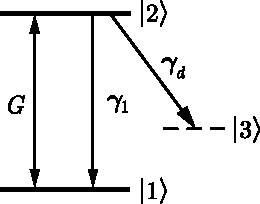
\includegraphics[width=4cm]{fig}
%  \caption{\label{f:fig}%
%  Подпись к рисунку.
%  }
%\end{figure}

%\begin{wrapfigure}{r}{0.35\textwidth}
%\centering
%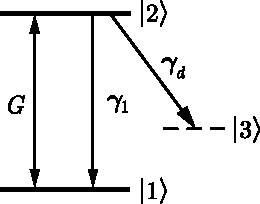
\includegraphics[width=4cm]{fig}
%\caption{\label{f:ff}%
%Рисунок <<в оборку>>.
%}
%\end{wrapfigure}

%Если разность энергий электронно-дырочных уровней $E_2 - E_1$ близка к энергии продольного оптического фонона $\hbar\Omega_{\mathrm{LO}}$, то в разложении волновых функций полного гамильтониана можно ограничиться нулевым приближением для всех состояний, за исключением близких по значению к $E_2$.
%Волновые функции последних представляют собой следующие комбинации вырожденных состояний\footnote{Текст сноски}.

%Ссылка на таблицу~\ref{t:InPSiO2}.
%\begin{table}[!ht]
%  \centering
%  \caption{Пример таблицы}\label{t:InPSiO2}
%  \begin{tabular}{l|ccc}
%    \hline\hline
%    & \quad$\lambda \cdot 10^{-11}$,~$\text{дин}\cdot\text{см}^{-2}$
%    & \quad$\mu \cdot 10^{-11}$,~$\text{дин}\cdot\text{см}^{-2}$
%    & \quad$\rho$, $\text{г}\cdot\text{см}^{-3}$ \\
%    \hline
%    InP       & 3.82 & 1.69 & 4.14 \\
%    SiO$_{2}$ & 1.57 & 3.11 & 2.2  \\
%    \hline\hline
%  \end{tabular}
%\end{table}

%\begin{figure}[!ht]
%  \centering
%  \begin{minipage}{5cm}
%    \centering
%    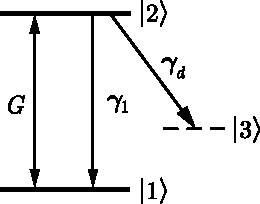
\includegraphics[width=4cm]{fig}
%    \caption{Рисунок с отдельным названием}
%  \end{minipage}
%  \quad
%  \begin{minipage}{5cm}
%    \centering
%    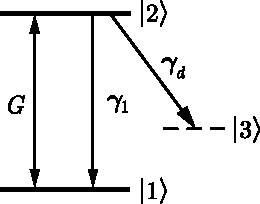
\includegraphics[width=4cm]{fig}
%    \caption{Рисунок с отдельным названием}
%  \end{minipage}
%  \quad
%  \begin{minipage}{5cm}
%    \centering
%    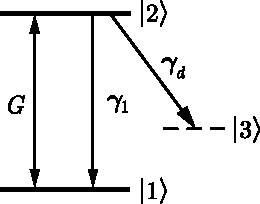
\includegraphics[width=4cm]{fig}
%    \caption{Рисунок с отдельным названием}
%  \end{minipage}
%\end{figure}

%\begin{figure}[!ht]
%  \centering
%  \begin{minipage}{5cm}
%    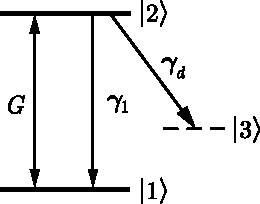
\includegraphics[width=4cm]{fig}
%  \end{minipage}
%  \begin{minipage}{5cm}
%    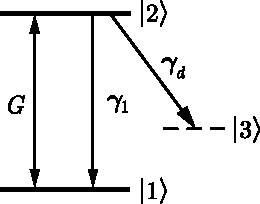
\includegraphics[width=4cm]{fig}
%  \end{minipage}
%  \caption{Рисунки с единым названием}
%\end{figure}

%Ссылка на внутренний рисунок (рис.~\ref{f:sub1}).

%\begin{figure}[!ht]
%\centering
%  \begin{minipage}{5cm}
%    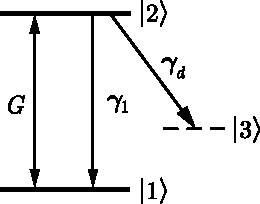
\includegraphics[width=4cm]{fig}\subcaption{}\label{f:sub1}
%  \end{minipage}
%  \begin{minipage}{5cm}
%    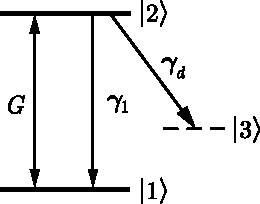
\includegraphics[width=4cm]{fig}\subcaption{}\label{f:sub2}
%  \end{minipage}
%  \begin{minipage}{5cm}
%    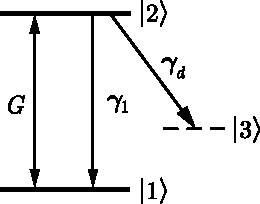
\includegraphics[width=4cm]{fig}\subcaption{}\label{f:sub3}
%  \end{minipage}
%  \caption[]{%
%  Рисунки с единым названием и подчиненной нумерацией:
%    \subref{f:sub1} ссылка 1,
%    \subref{f:sub2} ссылка 2,
%
%    \subref{f:sub3} ссылка 3.
%  }
%\end{figure}

%\subsection{Название подсекции}
%Текст подсекции
%\subsubsection{Название под-подсекции}
%Текст под-подсекции
%\paragraph{Название параграфа.}
%Текст параграфа
%\subparagraph{Название подпараграфа.}
%Текст подпараграфа

%Нумеруемый список:
%\begin{enumerate}
%  \item Первый уровень вложенности.
%  \begin{enumerate}
%    \item Второй уровень вложенности.
%    \begin{enumerate}
%      \item Третий уровень вложенности.
%    \end{enumerate}
%  \end{enumerate}
%\end{enumerate}

%Демонстрация полностью настраиваемых окружений типа <<теорема>>.

%\newtheorem{theorem}{Теорема}[chapter]
%\def\theoremstyle{}
%\def\postthetheorem{:}

%\newtheorem{lemm}{Лемма}[chapter]
%\def\thelemmstyle{\bfseries}
%\def\oparglemmstyle{}
%\def\lemmstyle{}
%\def\preoparglemm{(}
%\def\postoparglemm{):}

%\newtheorem{remark}{Примечание}[chapter]
%\def\remarkstyle{\itshape}
%\def\theremarkstyle{}
%\def\posttheremark{:}

%\begin{lemm}[Шура]
%Квадратная матрица, коммутирующая со всеми матрицами неприводимого представления, кратна единичной.
%\end{lemm}

%\begin{theorem}
%Гомоморфный образ группы изоморфен фактор-группе по ядру гомоморфизма.
%\end{theorem}

%\begin{remark}
%Текст примечания.
%\end{remark}

% Глава 2
%!TEX root = thesis.tex"`

\chapter{Модель взаимодействующего электронного газа на однородном компенсирующем фоне}

\section{Классическая модель однокомпонентной плазмы}
Классическая модель однокомпонентной плазмы (\acrshort{okp}) ~--- это модель точечных ионов, помещенных для обеспечения электронейтральности в равномерно распределенную среду заряда противоположного знака.
% TODO: Не уверен, стоит ли оставлять примеры
Такая модель является хорошим приближением для плазмы сверхвысоких давлений, реализующихся, например, в центре белых карликов и тяжелых планет типа Юпитера.
В этих случаях под действием давления вещество полностью ионизовано, а вырожденные электроны обладают достаточной кинетической энергией $\epsilon_k \approx \epsilon_F$, чтобы образовать почти однородное фоновое распределение зарядовой плотности.
Модель \acrshort{okp} является простейшей нетривиальной моделью плазмы, так как вид потенциала взаимодействия здесь не вызывает сомнений, а отсутствие квантовых эффектов позволяет исключить из рассмотрения образование связанных состояний (молекул, атомов, ионов) и влияние вырождения и интерференции. Важным свойством модели \acrshort{okp} является зависимость ее свойств только от одного параметра $\gamma = q_i^2/(kT\bar{r})$ в силу однородности кулоновского потенциала, где $q_i$~--- заряд иона, $\bar{r}$~--- среднее расстояние между ионами, обычно определяемое соотношением $4\pi\bar{r}^3/3 = 1/n_i$, $n_i$~--- концентрация ионов.  Более подробно с моделью и ее основными результатами можно ознакомиться в \cite{Fortov:neid_plasma}.

Большое количество результатов по \acrshort{okp} получено методом Монте-Карло.
Основным параметром в этих результатах является бинарная корреляционная функция $g(r)$.
На ее основании возможно вычислить внутреннюю энергию:
\begin{equation}
    \label{eq:internal_energy_g}
    u=3 n_{\mathrm{i}} k T / 2+u_{\text{кор}},
\end{equation}
\begin{equation}
    \label{eq:u_corr_g}
    u_{\text{кор}} /\left(n_{\mathrm{i}} k T\right)=\left(n_{\mathrm{i}} / 2 k T\right) \int d \mathbf{r}\left(Z^{2} e^{2} / r\right)[g(r)-1].
\end{equation}

Результаты вычислений методом Монте-Карло для $1 \leq \gamma \leq 160$ были аппроксимированы в \cite{Slattery:u_corr_approximation} с погрешностью $3 \cdot 10^{-5}$ следующим выражением:
\begin{equation}
    \label{eq:u_corr_approx}
    u_{\text{кор}} /\left(n_{\mathrm{i}} k T\right)=a \gamma+b \gamma^{1 / 4}+c \gamma^{-1 / 4}+d
\end{equation}
где $a=-0,89752$, $b=0,94544$, $c=0,17954$, $d=-0,80049$.

Давление можно получить по теореме вириала $p V = u/3$.
\begin{equation}
    \label{eq:p_approx}
    p = \cfrac{u}{3V}
    = \cfrac{n_\mathrm{i} kT}{3V} \left( \frac{3}{2}
    + a \gamma + b \gamma^{1/4} + c \gamma^{-1/4} + d \right)
\end{equation}
Интегрируя \eqref{eq:u_corr_approx} по $\gamma$, можно получить свободную энергию \acrshort{okp}:
\begin{multline}
    \label{eq:f-density-gas-approx}
    f=F /\left(n_{\mathrm{i}} k T\right) = \\
    =a \gamma+4\left(b \gamma^{1 / 4}-c \gamma^{-1 / 4}\right)+(d+3) \ln \gamma-(a+4 b-4 c+1,135)
\end{multline}

Заметим, что в соответствии с \eqref{eq:p_approx} высокое значение $\gamma$ приводит к отрицательному давлению компонента (поскольку $a < 0$).
Это не приводит к неустойчивости \acrshort{okp}: полное давление оказывается положительным за счет большого давления электронного газа.

Для \acrshort{okp} возможно явление кристаллизации, впервые рассмотренное Вигнером в \cite{Wigner:plasma_condensation}.
Было показано, что классический электронный газ с концентрацией $n_e$ на фоне компенсирующего заряда должен при достаточно низких концентрациях образовывать упорядоченную структуру.
Это вызвано тем, что стабилизирующая решетку кулоновская энергия $V_{\mathrm{C}} \sim e^{2} n_{\mathrm{e}}^{1 / 3} \sim e^{2} / \bar{r}$ при расширении плазмы уменьшается медленнее, чем разрушающая решетку кинетическая энергия $\varepsilon_\text{к} \sim \varepsilon_{F} \sim \hbar^{2} n_{\mathrm{e}}^{2 / 3} / 2 m$.
Поэтому при малых плотностях кинетическая энергия $\varepsilon_\text{к} \sim n_{\mathrm{e}}^{2 / 3}$ становится меньше потенциальной $V_{\mathrm{C}} \sim n_{\mathrm{e}}^{1 / 3}$ и не способна разрушить упорядоченную структуру электронов, возникшую из-за отталкивания.

В работе \cite{Slattery:u_corr_approximation} были получены результаты вычислений для кристаллической \acrshort{okp} с объемно-центрированной решеткой. Избыточная энергия при $160~\lesssim~\gamma~\lesssim~300$ в \cite{Slattery:u_corr_approximation} аппроксимирована выражением:
\begin{equation}
    \label{eq:u_corr_solid_approx}
    u_{\text{кор}} / n_{\mathrm{i}} k T=a_{\mathrm{BCC}} \gamma+\frac{3}{2}\, b \gamma^{-2}=0,895929 \gamma+1,5+2980 / \gamma^{2}
\end{equation}
Из выражения \eqref{eq:u_corr_solid_approx} следует выражение для плотности свободной энергии решетки:
\begin{equation}
    \label{eq:f-density-solid-approx}
    f(\gamma)=-0,895929+9 \gamma / 2-1,8856-1490 / \gamma^{2}.
\end{equation}
Зависимости свободных энергий газовой \eqref{eq:f-density-gas-approx} и твердой \eqref{eq:f-density-solid-approx} фаз пересекаются при $\gamma_m = 165$ \cite{Slattery:u_corr_approximation}.
При этом значении параметра неидеальности происходит вигнеровская кристаллизация \acrshort{okp}.

\section{Суммирование Эвальда}
\label{sec:ewald}
Для расчета энергии в системах с дальнодействующими потенциалами широко используется метод суммирования по Эвальду \cite{ewald:summation_original}.
В данном методе потенциал взаимодействия разбивается на два слагаемых: короткодействующее и дальнодействующее.
Первое слагаемое вычисляется в действительном пространстве, в то время как для расчета второго используется преобразование Фурье.
По сравнению с прямым подсчетом данный метод дает быструю сходимость по энергии, что обеспечивает высокую точность и скорость расчетов.

Более подробно, в методе суммирования по Эвальду предлагается переписать потенциал взаимодействия $\phi(\vec{r})$ в виде:
\begin{equation}
    \label{eq:ewald:potention_def}
    \phi(\vec{r}) \eqdef \phi_{sr}(\vec{r})+\phi_{lr}(\vec{r}),
\end{equation}
где $\phi_{sr}(\vec{r})$ отвечает за короткодействующую часть, энергия которой быстро сходится, а $\phi_{lr}(\vec{r})$ соответствует дальнодействующей части, энергия которой суммируется в Фурье-пространстве.

Предполагается, что энергия короткодействующей части потенциала суммируется непосредственно и основная проблема состоит в суммировании дальнодействующего вклада в потенциал.
Также из-за использования Фурье-преобразования метод неявно подразумевает, что рассматриваемая система является бесконечно периодической, что является разумным предположением для кристаллических структур.

Будем называть примитивной ячейкой минимальную повторяющуюся часть периодической системы.
Также для определенности выберем одну ячейку и назовем ее \textit{центральной}, а остальные будем называть \textit{образами}.

Энергия дальнодействующего взаимодействия есть сумма энергий взаимодействия между зарядами центральной ячейки и всех остальных зарядов решетки.
Ее можно записать в виде:
\begin{equation}
    \label{eq:ewald:energy_lr}
    E_{lr}=\iint d \vec{r} d \vec{r'} \rho_{tot}(\vec{r}) \rho_{u c}\left(\vec{r'}\right) \phi_{lr}\left(\vec{r}-\vec{r'}\right),
\end{equation}
где введена плотность заряда примитивной ячейки $\rho_{uc} (\vec{r})$, представляющая из себя сумму по зарядам внутри \textit{одной} ячейки:
\begin{equation}
    \label{eq:ewald:rho_uc_def}
    \rho_{uc}(\vec{r}) \eqdef \sum_{\text{charges}\ k} q_{k} \delta\left(\vec{r}-\vec{r}_{k}\right)
\end{equation}
и суммарная плотность заряда $\rho_{tot}(\vec{r})$, представляющая из себя ту же сумму, но с добавлением зарядов от образов:
\begin{equation}
    \label{eq:ewald:rho_tot_def}
    \rho_{tot}(\vec{r}) \eqdef \sum_{n_{1}, n_{2}, n_{3}} \sum_{\text{charges}\,k} q_{k} \delta\left(\vec{r}-\vec{r}_{k}-n_{1} \vec{a}_{1}-n_{2} \vec{a}_{2}-n_{3} \vec{a}_{3}\right).
\end{equation}
Здесь $\delta (\vec{x})$ ---~ дельта-функция Дирака, $\vec{a_1}$, $\vec{a_2}$, $\vec{a_3}$ ---~ вектора решетки и $n_1$, $n_2$, $n_3$ пробегают по всем целым числам.

На \eqref{eq:ewald:rho_tot_def} можно смотреть как на свертку \eqref{eq:ewald:rho_uc_def} с \textit{функцией ячейки} $L (\vec{r})$:
\begin{equation}
    \label{eq:ewald:lattice_function_def}
    L(\vec{r}) \eqdef \sum_{n_{1}, n_{2}, n_{3}} \delta\left(\vec{r}-n_{1} \vec{a}_{1}-n_{2} \vec{a}_{2}-n_{3} \vec{a}_{3}\right).
\end{equation}
Для полученной свертки имеем:
\begin{equation}
    \label{eq:ewald:rho_tot_conv_prod}
    \tilde{\rho}_{tot}(\vec{k}) = \tilde{L}(\vec{k}) \tilde{\rho}_{u c}(\vec{k}),
\end{equation}
где тильдами обозначены Фурье-образы.

Для функции ячейки $L(\vec{r})$ Фурье-образ есть:
\begin{equation}
    \label{eq:ewald:lattice_function_image}
    \tilde{L}(\vec{k})=\frac{(2 \pi)^{3}}{\Omega} \sum_{m_{1}, m_{2}, m_{3}} \delta\left(\vec{k}-m_{1} \vec{b}_{1}-m_{2} \vec{b}_{2}-m_{3} \vec{b}_{3}\right),
\end{equation}
где $\vec{b_1} = \cfrac{\vec{a}_{2} \times \vec{a}_{3}}{\Omega}$, $\vec{b_2}$ и $\vec{b_3}$ получаются циклическими перестановками, индексы $m_1$, $m_2$, $m_3$ по-прежнему пробегают все целые числа и $\Omega$ есть объем центральной ячейки: $\Omega~=~\vec{a_1} \cdot (\vec{a_2} \times \vec{a_3})$.
Стоит заметить, что и $L (\vec{r})$, и $\tilde{L} (\vec{r})$ являются действительными четными функциями.

Вводя эффективный одночастичный потенциал
\begin{equation}
    \label{eq:ewald:v_def}
    v(\vec{r}) \eqdef \int d \vec{r'} \rho_{u c}\left(\vec{r'}\right) \phi_{lr}\left(\vec{r}-\vec{r'}\right),
\end{equation}
можно переписать \eqref{eq:ewald:energy_lr} в виде:
\begin{equation}
    \label{eq:ewald:energy_v_rewrite}
    E_{lr}=\int d \vec{r} \rho_{tot}(\vec{r}) v(\vec{r})
\end{equation}
Заметим, что \eqref{eq:ewald:v_def} тоже является сверткой, что позволяет записать:
\begin{equation}
    \label{eq:ewald:v_fourier_conv_prod}
    \tilde{V}(\vec{k}) \eqdef \tilde{\rho}_{uc}(\vec{k}) \tilde{\Phi}(\vec{k}),
\end{equation}
где, как и в \eqref{eq:ewald:rho_tot_conv_prod}, тильдами обозначены Фурье-образы и введен Фурье-образ \eqref{eq:ewald:v_def}:
\begin{equation}
    \label{eq:ewald:v_fourier}
    \tilde{V}(\vec{k})=\int d \vec{r} v(\vec{r}) e^{-i \vec{k} \cdot \vec{r}}.
\end{equation}

Согласно теореме Планшереля, суммирование для получения $E_{lr}$ можно провести в Фурье-пространстве, что дает:
\begin{multline*}
    E_{l r} = \int \frac{d \vec{k}}{(2 \pi)^{3}} \tilde{\rho}_{tot}^{*}(\vec{k}) \tilde{V}(\vec{k})
    = \int \frac{d \vec{k}}{(2 \pi)^{3}} \tilde{L}^{*}(\vec{k})\left|\tilde{\rho}_{u c}(\vec{k})\right|^{2} \tilde{\Phi}(\vec{k}) = \\
    = \frac{1}{\Omega} \sum_{m_{1}, m_{2}, m_{3}}\left|\tilde{\rho}_{u c}(\vec{k})\right|^{2} \tilde{\Phi}(\vec{k}),
\end{multline*}
\begin{equation}
    \label{eq:ewald:energy_final}
    E_{lr} = \frac{1}{\Omega} \sum_{m_{1}, m_{2}, m_{3}}\left|\tilde{\rho}_{u c}(\vec{k})\right|^{2} \tilde{\Phi}(\vec{k}),
\end{equation}
где в суммировании $\vec{k}=m_{1} \vec{b}_{1}+m_{2} \vec{b}_{2}+m_{3} \vec{b}_{3}$.

Формула \eqref{eq:ewald:energy_final} есть основной результат.
Фурье-образ $\tilde{\rho}_{uc} (\vec{k})$ можно подсчитать, к примеру, алгоритмами \acrshort{bpf} (\textit{англ.} \acrshort{fft}).
Если найден фурье-образ $\tilde{\rho}_{uc} (\vec{k})$, то суммирование (или интегрирование) по $\vec{k}$ становится простым и приобретает быструю сходимость.
Стоит отметить, что используемая примитивная ячейка должна быть электронейтральной во избежание бесконечных сумм.

На практике суммирование \eqref{eq:ewald:energy_final} ведется в конечном диапазоне значений $m_1$, $m_2$, $m_3$.
Благодаря особенностям метода отбрасывание остальных членов приводит к небольшой потере точности, однако значительно уменьшает вычислительное время.
Оценку возникающих из-за отбрасывания ошибок можно найти, например, в \cite{ewald:errors_study}.

\section{Гамильтониан модели \texorpdfstring{\acrshort{veg}}{ВЭГ}}
Взаимодействующий электронный газ (\acrshort{veg}) ---~ это физическая модель электронного газа, в которой учитывается электростатическое взаимодействие между всеми зарядами в системе.
В данной работе рассматривается важный частный случай этой модели~--- так называемая модель <<желе>>, в которой электронейтральность обеспечивается компенсирующим фоном положительного заряда с постоянной полностью (так, чтобы суммарный заряд системы был равен нулю). Фон предполагается однородным и несжимаемым.

\textit{При изложении данной главы будем использовать систему единиц СГС.}

Для модели <<желе>> из $N$ электронов, заключенных в объеме $V$, имеющих концентрацию $\rho (\vec{r}) = \sum_{i=1}^{N} \delta(\vec{r}-\vec{r_i})$ при концентрации фоновых зарядов $n(\vec{R}) = N/V$, гамильтониан имеет вид \cite{jel:mahan_hamiltonian}:

\begin{equation}
    \label{eq:jel:ham_four_sum}
    \hat{H}=\hat{H}_{e l}+\hat{H}_{b a c k}+\hat{H}_{e l-b a c k}.
\end{equation}
Здесь $\hat{H}_{e l}$ ---~ это электронный гамильтониан, состоящий из кинетической энергии и электрон-электронного отталкивания:
\begin{equation}
    \label{eq:jel:ham_el_def}
    \hat{H}_{e l}=\sum_{i=1}^{N} \frac{\hat{\vec{p}}_i^2}{2 m}+\sum_{i<j}^{N} \frac{e^{2}}{\left|\hat{\vec{r}}_{i}-\hat{\vec{r}}_{j}\right|}.
\end{equation}
%
$\hat{H}_{b a c k}$ есть гамильтониан положительного фонового заряда, описывающий его взаимодействие с самим собой. Усредненное значение $\hat{H}_{b a c k}$ есть:
\begin{equation}
    \label{eq:jel:ham_back_expect}
    \left\langle\hat{H}_{b a c k}\right\rangle
    = \frac{e^{2}}{2} \int_{V} d \vec{R} \int_{V} d \vec{R}' \frac{n(\vec{R}) n\left(\vec{R}'\right)}{\left|\vec{R}-\vec{R}'\right|}
    = \frac{N^{2}}{2 V} \lim _{\mathbf{q} \rightarrow 0} v_{q},
\end{equation}
где введена фурье-компонента кулоновского потенциала $v_{q}=\frac{4 \pi e^{2}}{q^{2}}$.
%
Вклад электростатического взаимодействия электрона с фоном описывается членом $H_{el-back}$:
\begin{multline}
    \label{eq:jel:ham_el-back_expect}
    \left\langle\hat{H}_{e l-b a c k}\right\rangle
    = -\int_{V} d \vec{r} \int_{V} d \vec{R}\, \frac{e^{2} \rho(\vec{r}) n(\vec{R})}{|\vec{r}-\vec{R}|} = {} \\
    = -\frac{N^{2}}{V} \lim _{\mathbf{q} \rightarrow 0} v_{q}
    = -2 \left\langle\hat{H}_{b a c k}\right\rangle.
\end{multline}

Для конечных систем результаты \eqref{eq:jel:ham_back_expect} и \eqref{eq:jel:ham_el-back_expect} получаются конечными, поскольку $q$ достигает отличное от нуля минимальное значение, зависящее от объема системы.

Для систем с периодическими граничными условиями суммирование кулоновского взаимодействия можно провести упомянутым выше методом Эвальда (см. раздел \ref{sec:ewald}).
Учтем также возможное размытие заряда относительно его равновесного положения в форме функции Гаусса \cite{jel:blinov}.

Введем потенциал в точке $\vec{r}$, создаваемый всей решеткой без одного лишь заряда $j$, но с учетом его образов:

\begin{equation}
    \label{eq:jel:phi_no_j}
    \phi_{-j}(\vec{r})=\frac{1}{\varepsilon} \sum_{\vec{n}} \sum_{i=1}^{N} {}^\prime \frac{q_{i}}{\left|\vec{r}-\vec{r}_{i}+\vec{n} L\right|},
\end{equation}
где штрих у суммы обозначает, что $i \neq j$ при $\vec{n} = 0$.
Здесь $q_i$ указан для того, чтобы получающиеся результаты не были привязаны к типам и значениям зарядов.
Используя выражения для полной энергии:
\begin{equation}
    \label{eq:jel:coloumb_energy}
    E = \frac{1}{2} \sum_{j=1}^{N} q_{j} \phi_{-j}\left(\vec{r}_j\right)
\end{equation}
и плотности заряда:
\begin{equation}
    \rho_{i}(\vec{r})=q_{i} \cdot \delta\left(\vec{r}-\vec{r}_{\mathrm{i}}\right),
\end{equation}
получим полную энергию в виде:
\begin{equation}
    \label{eq:jel:ewald_E_coloumb_total}
    E = \frac{1}{\epsilon} \sum_{\vec{n}} \sum_{i=1}^{N} \sum_{j=1}^{N} {}^\prime \iint \frac{\rho_{i}(\vec{r}) \cdot
    \rho_{j}\left(\vec{r}'\right)}{\left|\vec{r}-\vec{r}^{\prime}+\vec{n} L\right|} d^3 \vec{r}\, d^3 \vec{r}^{\prime}.
\end{equation}

Разбиваем заряды на части:
\begin{equation}
\label{eq:jel:rho_separation}
\begin{aligned}
    \rho_i (\vec{r}) & = \rho_i^S (\vec{r}) + \rho_i^L (\vec{r}), \\
    \rho_i^S (\vec{r}) & = q_i \delta(\vec{r} - \vec{r_i}) - q_i G_\sigma (\vec{r} - \vec{r_i}), \\
    \rho_i^L (\vec{r}) & = q_i G_\sigma (\vec{r} - \vec{r_i}),
\end{aligned}
\end{equation}
где введено гауссово размытие заряда
\begin{equation}
    \label{eq:jel:gauss_blur}
    G_\sigma (\vec{r}) = \frac{1}{(2\pi \sigma^2)^{3/2}} \exp \left[ - \cfrac{|\vec{r}|^2}{2\sigma^2} \right].
\end{equation}
Дисперсия здесь будет играть роль некоторого параметра.

Выражение для энергии \eqref{eq:jel:coloumb_energy} с учетом \eqref{eq:jel:rho_separation} перепишется в виде:
\begin{equation}
    \label{eq:jel:E_separation}
    E = \frac{1}{2} \sum_{i=1}^N q_i \phi_{-i}^S (\vec{r_i}) + \frac{1}{2} \sum_{i=1}^N q_i \phi^L (\vec{r_i}) - \frac{1}{2} \sum_{i=1}^N q_i \phi_i^L (\vec{r_i})
    = E^S + E^L - E^{self}.
\end{equation}

Уравнение Пуассона для случая, когда заряд распределен по функции Гаусса, может быть решено аналитически. Само уравнение имеет вид:
\begin{equation}
    \label{eq:jel:phi_poisson}
    \Delta \phi_i (\vec{r}) = - \frac{4\pi}{\epsilon}\, G_\sigma (\vec{r}),
\end{equation}
а его решение выражается через функцию ошибок $\mathrm{erf} (x) = \frac{2}{\sqrt{\pi}} \int_0^x e^{-t^2} dt$ следующим образом:
\begin{equation}
    \label{eq:jel:phi_solution}
    \phi_\sigma (r) = \frac{1}{\epsilon r}\, \mathrm{erf} \left( \frac{r}{\sqrt{2}\sigma} \right).
\end{equation}

Таким образом,
\begin{equation}
\label{eq:jel:phi_S_solution}
\begin{aligned}
    \phi_i^S (\vec{r}) &= \frac{1}{\epsilon} \frac{q_i}{|\vec{r} -\vec{r_i}|}\, \mathrm{erfc} \left[ \frac{|\vec{r} - \vec{r_i}|}{\sqrt{2} \sigma} \right], \\
    \phi_i^L (\vec{r}) &= \frac{1}{\epsilon} \frac{q_i}{|\vec{r} -\vec{r_i}|}\, \mathrm{erf} \left[ \frac{|\vec{r} - \vec{r_i}|}{\sqrt{2} \sigma} \right],
\end{aligned}
\end{equation}
где $\mathrm{erfc} (x) = 1 - \mathrm{erf} (x)$. Теперь, с учетом размытия, можно переписать $\phi^S_{-i} (\vec{r})$ в виде:
\begin{equation*}
    \phi_i^S (\vec{r}) = \frac{1}{\epsilon} \sum_\vec{n} \sum_{j=1}^N {}^\prime \frac{q_j}{| \vec{r} - \vec{r_j} + \vec{n}L |}\, \mathrm{erfc} \left( \frac{|\vec{r} - \vec{r_j} + \vec{n}L}{\sqrt{2} \sigma} \right),
\end{equation*}
а энергию:
\begin{equation*}
    E^S = \frac{1}{2} \sum_{i=1}^N q_i \phi_{-i}^S (\vec{r_i})
    = \frac{1}{2\epsilon} \sum_\vec{n} \sum_{i=1}^N \sum_{j=1}^N {}^\prime \frac{q_i q_j}{|\vec{r_i} - \vec{r_j} + \vec{n}L|}\, \mathrm{erfc} \left( \frac{|\vec{r_i} - \vec{r_j} + \vec{n}L|}{\sqrt{2}\sigma} \right).
\end{equation*}
Это выражение аналогично исходному лишь с той разницей, что сумма обрезается функцией $\mathrm{erfc}$, что упрощает расчет.

Используя $\mathrm{erfc} (x) \xrightarrow[x \rightarrow 0]{} \frac{2}{\sqrt{\pi}} x$, можно получить для $E^{self}$:
\begin{equation}
    \label{eq:jel:E_self_final}
    E^{self} = \frac{1}{\epsilon} \frac{1}{\sqrt{2} \sigma} \sum_{i=1}^N q_i^2.
\end{equation}

Таким образом, осталось посчитать третью, дальнодействующую, часть.
Как было отмечено в разделе \ref{sec:ewald}, дальнодействующая часть считается в обратном пространстве.

Записывая плотность заряда в виде суммы по всем зарядам системы, периодически повторяющимся в пространстве:
\begin{equation*}
    \rho^L (\vec{r}) = \sum_\vec{n} \sum_{j=1}^N q_j G_\sigma (\vec{r} - \vec{r_j} + \vec{n}L),
\end{equation*}
имеем для Фурье-образа:
\begin{equation*}
    \tilde{\rho}\,^L (\vec{k}) = \int_V \sum_{j=1}^N q_j G_\sigma(\vec{r} - \vec{r_j} + \vec{n}L) e^{-i\vec{k}\vec{r}} d \vec{r}
    = \sum_{j=1}^N q_j e^{-i \vec{k} \vec{r_j}} e^{-\sigma^2 k^2 / 2} d\vec{r}.
\end{equation*}
Здесь использован тот факт, что $k$ есть вектор обратной решетки и потому $\exp(-i \vec{k} \vec{n} L) = 1$.

Тогда для Фурье-образа потенциала имеем:
\begin{equation}
    \label{eq:jel:phi_L_fourier}
    \tilde{\phi}\,^L (\vec{k}) = \frac{4\pi}{\epsilon} \sum_{j=1}^N q_j e^{-i \vec{k} \vec{r_j}}\, \frac{ e^{-\sigma^2 k^2 / 2} }{ k^2 },
\end{equation}
а сам потенциал (через обратное преобразование):
\begin{equation}
    \label{eq:jel:phi_L_spatial}
    \phi^L (\vec{r}) = \frac{4\pi}{V \epsilon} \sum_{\vec{k} \neq 0} \sum_{j=1}^N \frac{q_j}{k^2}\, e^{i \vec{k} (\vec{r} - \vec{r_j})} e^{-\sigma^2 k^2 / 2}.
\end{equation}
Вклад члена с $\vec{k} = 0$ нулевой, так как полный заряд примитивной ячейки предполагается нулевым.
Для энергии $E^L$ получаем:
\begin{equation}
    \label{eq:jel:E_L_final}
    E^L = \frac{4\pi}{2V \epsilon} \sum_{\vec{k} \neq 0} \sum_{i=1}^N \sum_{j=1}^N \frac{q_i q_j}{k^2} e^{i \vec{k} (\vec{r_i} - \vec{r_j})} e^{-\sigma^2 k^2 / 2}.
\end{equation}

Определяя структурный фактор $S (\vec{k}) = \sum_{i=1}^N q_i e^{i\vec{k} \vec{r_i}}$, дальнодействующую часть энергии возможно переписать в виде:
\begin{equation}
    \label{eq:jel:E_L_from_S}
    E^L = \frac{4\pi}{2V \epsilon} \sum_{\vec{k} \neq 0} \frac{e^{-\sigma^2 k^2 /2}}{k^2} | S (\vec{k}) |^2
\end{equation}
и получить окончательное выражение для полной энергии:
\begin{equation}
\label{eq:jel:total_energy_final}
\begin{aligned}
    E &= E^S + E^L - E^{self} = \\
    &= \frac{1}{2 \epsilon} \sum_{\vec{n}} \sum_{i=1}^N \sum_{j=1}^N {}^\prime \frac{q_i q_j}{|\vec{r_i} - \vec{r_j} + \vec{n}L|}\, \mathrm{erfc} \left( \frac{ |\vec{r_i} - \vec{r_j} + \vec{n}L| }{ \sqrt{2} \sigma } \right) + \\
    &+ \frac{4\pi}{2V \epsilon} \sum_{\vec{k} \neq 0} \frac{e^{-\sigma^2 k^2 / 2}}{k^2} | S (\vec{k}) |^2 - \frac{1}{\epsilon} \frac{1}{\sqrt{2\pi} \sigma} \sum_{i=1}^N q_i^2.
\end{aligned}
\end{equation}

Собирая результаты воедино, получим гамильтониан модели ВЭГ:
% TODO: (a.kozharin) Подумать, как собрать эту солянку из трех статей в один гамильтониан <- Mon Jun 22 00:30:13 2020
\begin{multline}
    \label{eq:jel:ham_final}
        \hat{H} = \sum\limits_{i=1}^{N} \cfrac{\hat{\vec{p}}_{i}^2}{2m}\, +
        \frac{1}{2 \epsilon} \sum_{\vec{n}} \sum_{i=1}^N \sum_{j=1}^N {}^\prime \frac{q_i q_j}{|\hat{\vec{r}}_i - \hat{\vec{r}}_j + \hat{\vec{n}}L|}\, \mathrm{erfc} \left( \frac{ |\hat{\vec{r}}_i - \hat{\vec{r}}_j + \hat{\vec{n}}L| }{ \sqrt{2} \sigma } \right) + {} \\
        {} + \frac{4\pi}{2V \epsilon} \sum_{\vec{k} \neq 0} \frac{e^{-\sigma^2 k^2 / 2}}{k^2} | \hat{S} (\vec{k}) |^2 - \frac{1}{\epsilon} \frac{1}{\sqrt{2\pi} \sigma} \sum_{i=1}^N q_i^2.
\end{multline}
Здесь $\hat{S} (\vec{k}) = \sum\limits_{i=1}^{N} q_{i} e^{i \vec{k} \hat{\vec{r}}_{i}}$, а оператор $\hat{\vec{n}}L$ соответствует координатному сдвигу на целое число ячеек.

\section{Усреднение по направлениям и изотропная модель \texorpdfstring{\acrshort{veg}}{ВЭГ}}
Непосредственное суммирование по Эвальду в том виде, который приведен в секции \ref{sec:ewald}, имеет два практических недостатка:
\begin{enumerate}
    \item Вычислительная сложность (нагрузка на процессор компьютера) быстро растет с ростом числа частиц в главной ячейке (как $N^2$).
    \item Комбинирование дальнодействующего кулоновского взаимодействия с периодическими граничными условиями может привести к появлению неизотропического электрического поля, имеющего кубическую симметрию в кристаллической решетке, составленной из главных ячеек.
        В этом смысле любая процедура суммирования кулоновских сил может считаться подходящей лишь в том случае, если погрешность результата, вызванная этой искуственной симметрией, пренебрежимо мала.
\end{enumerate}
В \cite{jel:pre-averaged_summation} предлагается новый метод суммирования, основанный на предварительном усреднении вдоль всех направлений главной ячейки.
Предполагается, что ячейка имеет вид куба с объемом $V = L^3$ и на систему наложены периодические граничные условия вместе с условиями электронейтральности.

Для начала заметим, что подбором параметра размытия $\sigma$ можно добиться возможности отбросить значительную часть членов суммирования в \eqref{eq:jel:total_energy_final} \cite{rapaport:terms_cutoff}.
В дальнейшем будем предполагать, что используемый параметр размытия позволяет нам осуществить указанное упрощение.

Приведем \eqref{eq:jel:total_energy_final} к виду, полученному в оригинальной работе Эвальда \cite{ewald:summation_original}.
Для этого необходимо сделать замену $\delta = \frac{\sqrt{2} \pi}{\sigma}$, а $| S (\vec{k}) |^2$ явно раскрыть с выделением тригонометрических функций.
Рассматривая энергию кулоновского взаимодействия $N$ ионов в главной ячейке, получим:
\begin{equation}
    \label{eq:mean:E_coloumb_main-cell}
    E_N = \sum\limits_{i=1}^{N} q_i \phi (\vec{r}_{i}),
\end{equation}
где $\phi (\vec{r}_{i})$ ---~ электростатический потенциал $i$-го иона в точке $\vec{r}_{i}$.
% TODO: (a.kozharin) Вот тут мы просто прыгаем к виду Эвальда. Нет, выкладки стоит самому провести и проверить, если останется время. Но, мне кажется, если считать только энергию главной ячейки и уйти на обозначения Эвальда, то должно быть все ок <- Mon Jun 22 23:53:31 2020
Согласно \cite{ewald:summation_original}, $\phi$ имеет вид:
\begin{equation}
    \label{eq:mean:phi_as_sum}
    \phi (\vec{r}_{i}) = \phi_1 (\vec{r}_{i}) + \frac{1}{2}\, \sum\limits_{j \neq i}^{N} \phi_2 (\vec{r}_{i}, \vec{r}_{j}),
\end{equation}
где в отстутствии внешнего поля $\phi_1$ есть константа:
\begin{equation}
    \label{eq:mean:phi_1}
    \phi_1 = \cfrac{q_{i}}{L}\, \left( \frac{1}{2\pi}\, \sum\limits_{n > 0}^{} \frac{1}{n^2}\, e^{-\pi^2 n^2 / \delta^2} - \cfrac{\delta}{\sqrt{\pi}}\, \right),
\end{equation}
а парный потенциал получается следующим:
\begin{equation}
    \label{eq:mean:phi_2}
    \phi_2 = q_{j} \left[ \frac{1}{r_{ij}}\, \mathrm{erfc} \left( \delta \cfrac{r_{ij}}{L}\, \right) + \frac{1}{2\pi L}\, \sum\limits_{\vec{n} > 0}^{} \frac{1}{n^2}\, e^{-\pi^2 n^2 / \delta^2} \cos \left( \frac{2\pi}{L}\, \vec{n} \cdot \vec{r}_{ij} \right) \right].
\end{equation}
Здесь $\vec{n} / L$ есть трехмерный взаимный вектор решетки ($n = | \vec{n} |$), $\vec{r}_{ij} = \vec{r}_{i} - \vec{r}_{j}$, $r_{ij} = |\vec{r}_{ij}|$.
Параметр $\delta / L$ обычно называют параметром Эвальда.

Учитывая, что все направления главной решетки в изотропической жидкости должны быть равноправны, обе части \eqref{eq:mean:phi_2} можно усреднить вдоль всех всех направлений вектора $\vec{n}$.
Обозначая $\phi_2 (r_{ij}) \equiv \langle \phi_2 (\vec{r}_{ij}) \rangle$, получим:
\begin{equation}
    \label{eq:mean:phi_2_averaged}
    \phi_2 (r_{ij}) = \frac{q_{j}}{r_{ij}} \left[ \mathrm{erfc} \left( \delta \cfrac{r_{ij}}{L}\, \right) + \frac{1}{2\pi^2}\, \sum\limits_{\vec{n} > 0}^{} \frac{1}{n^3}\, e^{-\pi^2 n^2 / \delta^2} \sin \left( \frac{2\pi}{L}\, n r_{ij} \right) \right].
\end{equation}
Поскольку $\mathrm{erfc}(x) - 1$ и $\sin (x)$ являются нечетными функциями, возможно следующее разложение в ряд:
\begin{equation}
    \label{eq:mean:phi_2_series}
    \phi_2 (r_{ij}) = \cfrac{q_{j}}{r_{ij}}\, \left( 1 + \sum\limits_{k \geq 0}^{} C_{k} r_{ij}^{2k+1} \right),
\end{equation}
где коэффициенты $C_k$ можно найти прямым разложением в ряд Маклорена \eqref{eq:mean:phi_2_averaged} с использованием формулы Эйлера-Маклорена, обобщенной на случай суммирования по трехмерному пространству.
Это в результате даст \cite{jel:pre-averaged_summation}:
\begin{equation}
    \label{eq:mean:C_coeffs}
    \begin{aligned}
        C_0 &= \frac{1}{\pi}\, \sum\limits_{\vec{n} > 0}^{} \frac{1}{n^2}\, e^{-\pi^2 n^2 / \delta^2} - \frac{2\delta}{\sqrt{\pi}}\, \\
        C_1 &= \frac{2\pi}{3 L^3}\, \\
        C_k &= 0, \quad k > 1
    \end{aligned}
\end{equation}
Если теперь учесть условие электронейтральности, то окажется, что член в \eqref{eq:mean:phi_2_series}, не зависящий от расстояния (пропорциональный $C_0$), уничтожает вклад от $\phi_1$ в \eqref{eq:mean:phi_as_sum}.
Это означает, что суммарная энергия кулоновского взаимодействия в главной ячейке может быть описана суммой $E_N = \sum_{i=1}^N \phi (r_{ij})$, где
\begin{equation}
    \label{eq:mean:phi_final}
    \phi (r_{ij}) = \frac{q_i q_j}{r_{ij}}\, \left[ 1 + \frac{1}{2}\, \left( \frac{r_{ij}}{r_{m}} \right)^3 \right]
\end{equation}
и $r_{m} = (3 / 4 \pi)^{1 / 3} L$ ---~ радиус эквивалентной по объему сферы главной ячейки: $\frac{4}{3} \pi r_{m}^3 = L^3$.

Результат \eqref{eq:mean:phi_final} и есть усредненный по направлениям потенциал.
Он обладает следующими свойствами:
\begin{enumerate}
    \item Он стремится к чистому кулоновскому парному потенциалу при малых межионных расстояниях;
    \item Его первая производная равна нулю в $r_{m}$;
    \item Его значение в минимуме $r = r_m$ отлично от нуля и равно $\phi (r_m ) = 3 q_i q_j / 2 r_m$.
\end{enumerate}

Значение потенциала в точке $r_m$ можно обнулить, прибавив к нему постоянную добавку $-\phi (r_m)$.
Воспользовавшись условием электронейтральности, получаем окончательное выражение суммарной кулоновской энергии главной ячейки в следующем виде:
\begin{equation}
    \label{eq:mean:E_coloumb_main-cell_final}
    E_N = - \sum\limits_{i=1}^{N} \frac{3q_{i}^2}{4\pi r_m}\, + \frac{1}{2}\, \sum\limits_{i=1}^{N} \sum\limits_{j=1, j \neq i}^{N} \tilde{\phi} (r_{ij}),
\end{equation}
где
\begin{equation}
    \label{eq:mean:phi_tilde}
    \tilde{\phi} (r) =
    \begin{cases}
        \cfrac{q_i q_j}{r}\, \left\{ 1 + \cfrac{1}{2}\, \left( \cfrac{r}{r_m}\,  \right) \left[ \left(\cfrac{r}{r_m}\,   \right)^2 - 3 \right] \right\}, \quad r < r_m \\
        0, \quad r \geq r_m
    \end{cases}
\end{equation}
есть эффективный потенциал межионного взаимодействия, который равен нулю вместе со своими производными в $r_m$ и таковым остается при $r > r_m$.

Объединяя полученное выражение с кинетической энергией, получим \textit{гамильтониан изотропной модели \acrshort{veg}}:
\begin{equation}
    \label{eq:mean:ham_final}
    \hat{H} = \sum\limits_{i=1}^{N} \frac{\hat{\vec{p}}_{i}^2}{2m}\, - \sum\limits_{i=1}^{N} \frac{3q_{i}^2}{4\pi \hat{r}_m}\, + \frac{1}{2}\, \sum\limits_{i=1}^{N} \sum\limits_{j=1, j \neq i}^{N} \tilde{\phi} (\hat{r}_{ij}),
\end{equation}

% Глава 3
\chapter{Программная реализация метода функционала плотности для модели ВЭГ}

\section{Метод функционала электронной плотности}

\section{Метод функционала плотности для модели ВЭГ}

\section{Алгоритм моделирования ВЭГ методом функционала плотности при конечной температуре}


% Заключение
%!TEX root = thesis.tex"`

\conclusion

В работе получены следующие основные результаты:

\begin{enumerate}
    \item Получены аналитические выражения для вторых производных термодинамического потенциала и термодинамических коэффициентов \acrshort{ifg}.
    \item Получены асимптотические выражения для всех термодинамических функций \acrshort{ifg} в пределе низких и высоких температур.
    \item Разработана общедоступная программная реализация для модели \acrshort{ifg} на языке \Gls{python}.
    \item Получен гамильтониан изотропной модели \acrshort{veg}.
    \item Разработан алгоритм программной реализации \acrshort{mfp} для модели \acrshort{veg}.
\end{enumerate}

% Список литературы
\printbibliography[heading=bibintoc]
\printglossaries

% Приложения
\appendix
\chapter{Пример расчета термодинамических свойств ИФГ}


\end{document}
